% Not sure where this fits within the overall thing anymore...


\section{melcomp\_3}

Following discussions with Laurence Maloney at the Visual Neuroscience Summer School about this work, and about his own work on colour constancy \citep{maloney_computational_1984,maloney_color_1986}, Laurence suggested a simple game: \emph{``Given cone catches from an unknown surface under an unknown illuminant, guess the illuminant. If you are able to guess the illuminant with a moderate accuracy, you've cracked colour constancy.''}

Whilst this had been an implicit thread throughout much of the work to this point, it was a neat idea to be spelled out so clearly. A reservation however, was that based on my experience with the rotational corrective transform (Figure \ref{fig:viewpoint}), it had been shown that a correction (to an illuminant-independent space) seemed possible even without explicit knowledge of the illuminant. Of course one could get an estimate of the illuminant from such a computation, but it was a potential output, not a requisite input. All the same, it was believed that solving Laurence's game with a melanopic signal would be relatively trivial.

In melcomp\_3 this was attempted, using the framework of linear modelling which Laurence is so well known for. It was used in a relatively rudimentary way, compared to the complex manner in which Laurence uses it in his thesis \citep{maloney_computational_1984}. Whereas there it is used to compute a solution to colour constancy, here it is only used it to define the light sources, and then query which signals can predict the light sources so defined.

The script starts in much the same way as in melcomp\_1 and 2, by loading data upon which to perform the computations. This time, an extended subset of the \citet{vrhel_measurement_1994} dataset is used, considering anything which could be considered natural rather than the small selection previously needed, on the basis that to consider correlation having an increased number of datapoints would be beneficial. At this stage the \gls{SP} fundamentals were used, mainly in order to obey the rules of the traditional \gls{MB} diagram \citep{macleod_chromaticity_1979}. Again the Granada data \citep{hernandez-andres_color_2001} was ussed. From these inputs, $[L,M,S,R,I]$ values were computed, along with the corresponding \gls{MB} chromaticity values and pseudo-MB values ($i_{\text{MB}}$ and $r_{\text{MB}}$) for each surface under each illuminant.

The principal component representation of each illuminant was also calculated. A variable weighting was specified, which gave most importance to wavelengths between the peak sensitivity of the S-cones and the peak sensitivity of the L-cones, before tailing off at each end (shown in Figure \ref{fig:VW}). This weighting is an important and difficult choice, and no entirely sensible solution is forthcoming\footnote{Do we care more about certain wavelengths than others? Yes. Which ones and by how much by? Unknown, and evolutionarily circular.}. \citet{maloney_evaluation_1986} discusses this further. %read and say more

\begin{figure}[htbp]
 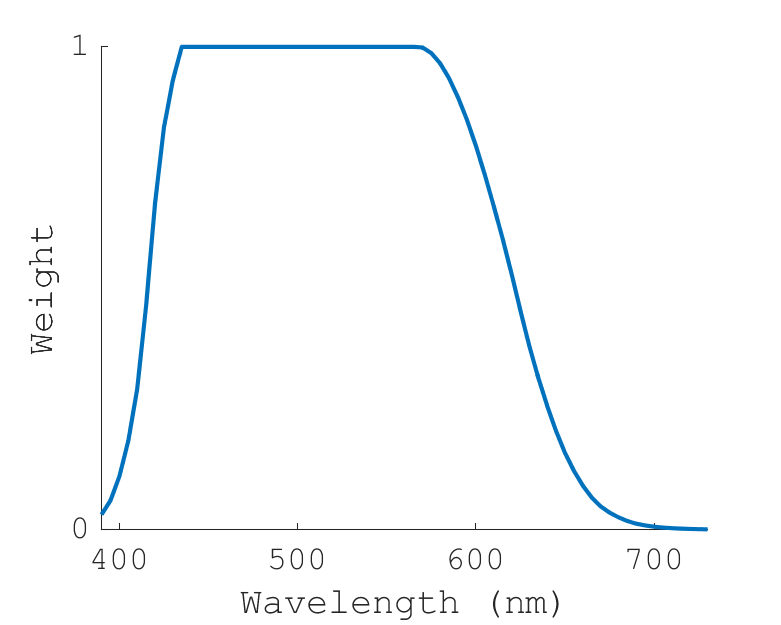
\includegraphics[max width=\textwidth]{figs/comp/melcomp_3/vw.png}
 \caption{The variable weightings applied during the \gls{PCA} analysis. Generated by tracing the upward ramp of the S-cone sensitivity being used, plateauing at unity until the decrease of the L-cone sensitivity, and then following the decrease of the L-cone sensitivity.}
 \label{fig:VW}
\end{figure} 

The principal components identified are shown in Figure \ref{fig:PCA}. The first three components account for 99.952\%, 0.037\% and 0.005\% of variance respectively.

\begin{figure}[htbp]
 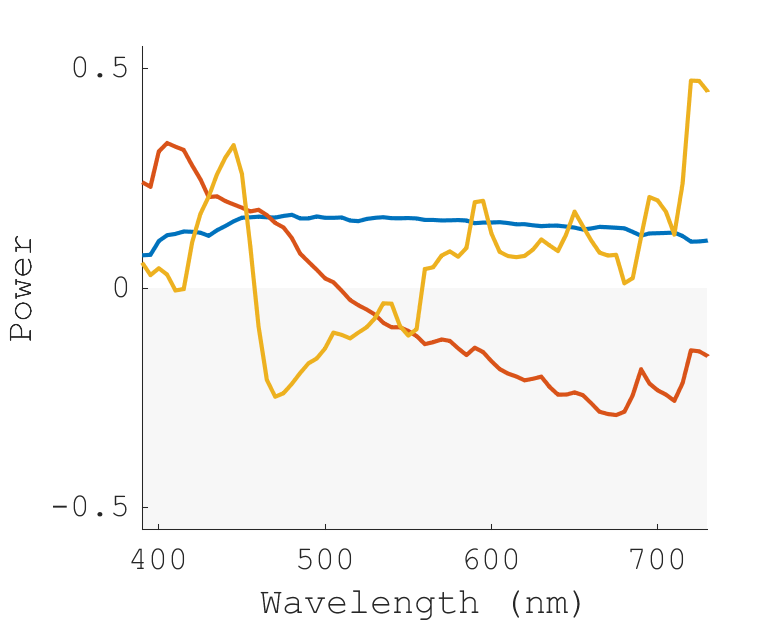
\includegraphics[max width=\textwidth]{figs/comp/melcomp_3/8.png} %legend required
 \caption{The first 3 principal components for the Granada daylight dataset, conditional on the variable weighting shown in Figure \ref{fig:VW}.}
 \label{fig:PCA}
\end{figure} 

% Might be neat to show the chromatic effect of each of these PCs?

The correlation was then computed for a large number of candidate signals and the scores for different components of the \glspl{SPD}. This is shown in \ref{fig:19}. Simply put, this is a way to ask: which signal was best at predicting each element of the daylight spectra upon a scene? It can be seen that $L$, $M$, $S$, $R$ and $I$ (along with all other simple additive combinations - `$L+M$', `$SP\_lum$' and `$r+i$') all have very high correlation with the first principal component score. This fundamentally reflects the high amount of variance accounted for my the \gls{PC1} for this daylight dataset - a simple sensor at almost any point in the spectrum will be able to approximate very well the score for this principal component. An example of data and a fit for this is shown in Figure \ref{fig:L-PC1}.

The ability of any of these signals to predict second or higher principal component scores is considerably poorer, and to identify which, if any, are successful the plot on the left of Figure \ref{fig:19} needs to be normalised (by column). The normalised result is shown on the right of the same figure. From this it can be seen that `$S/I$' has the highest correlation, which is particularly interesting considering the discussions at the end of the melcomp\_2, which highlighted the potential of a relationship between s-cone signals and melanopic signals.

\begin{figure}[htbp]
 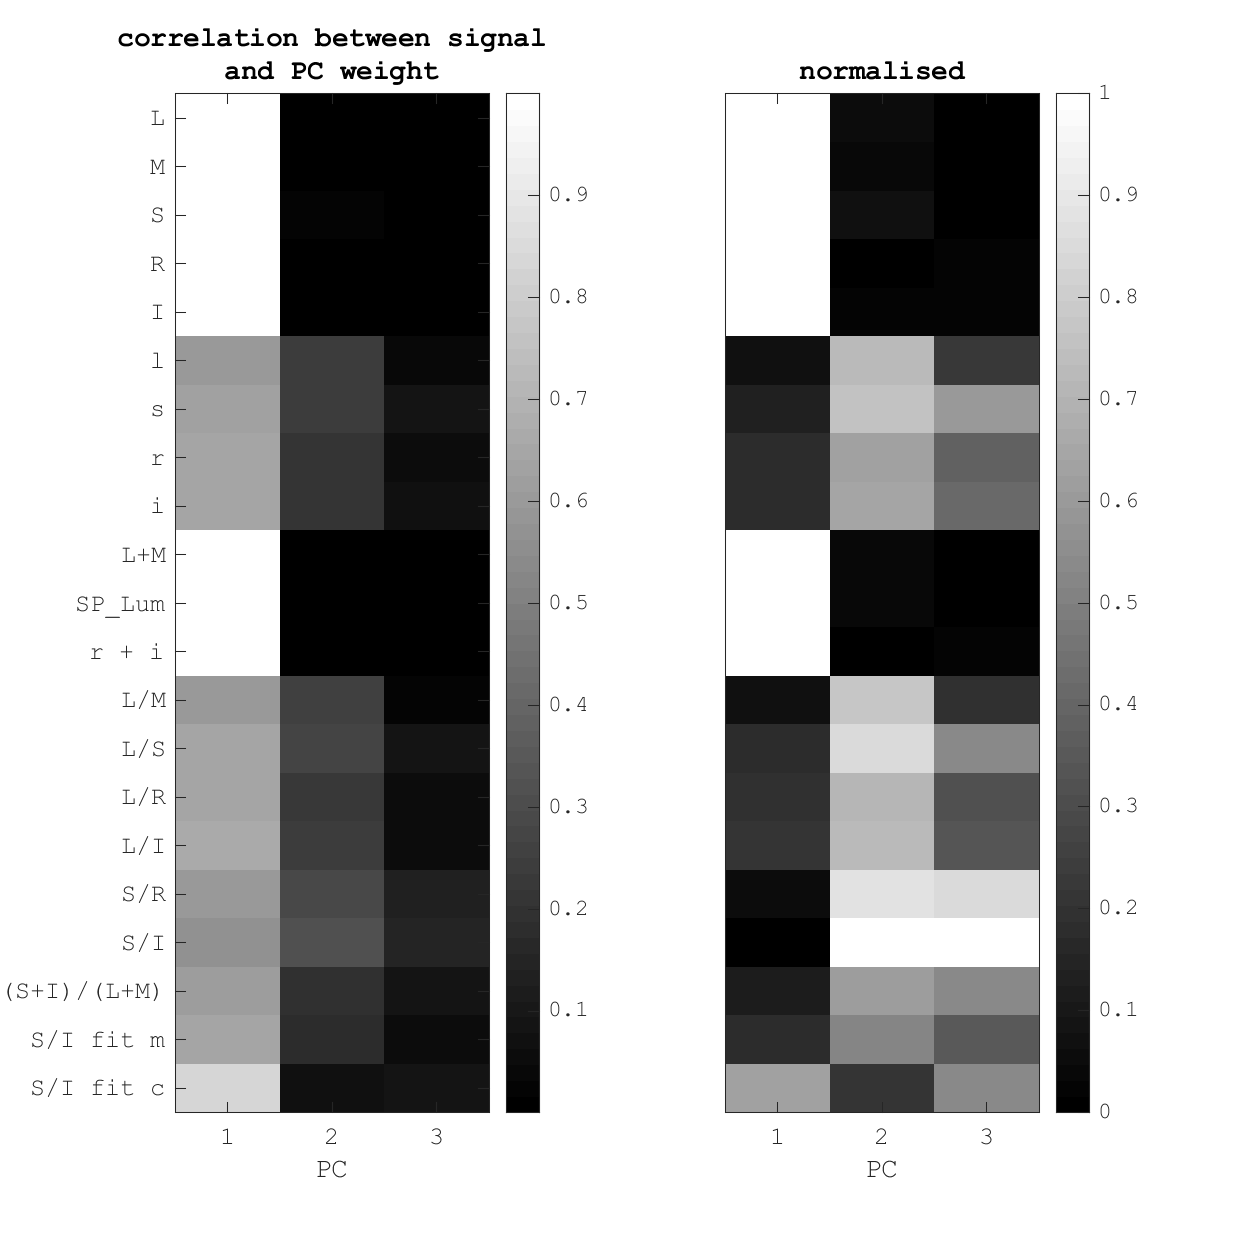
\includegraphics[max width=\textwidth]{figs/comp/melcomp_3/19.png}
 \caption{Correlation coefficients between a range of signals and the first three principal component scores. On the left of a raw representation, and on the right each column is normalised between 0 and 1.}
 \label{fig:19}
\end{figure} 

Looking more closely at the data underlying these correlations it can be seen that whereas the relationships for \gls{PC1} is simple (Figure \ref{fig:L-PC1}), the relationship between `$S/I$' and the \gls{PC2} is rather less simple (Figure \ref{fig:S/I-PC2}). Further examination showed that this relationship was dependent upon the PC1 value, and that by including an $L$ component (considered a biologically accessible correlate to \gls{PC1} score), a much more robust relationship could be produced. This is demonstrated in Figure \ref{fig:withPC1}. The additional value need not be $L$, and could be any other primary signal. Using each primary signal in turn instead of $L$ yields correlation coefficients of 0.916, 0.922, 0.929, 0.921 and 0.924 respectively (all high, $S$ highest).

\begin{figure}[htbp]
 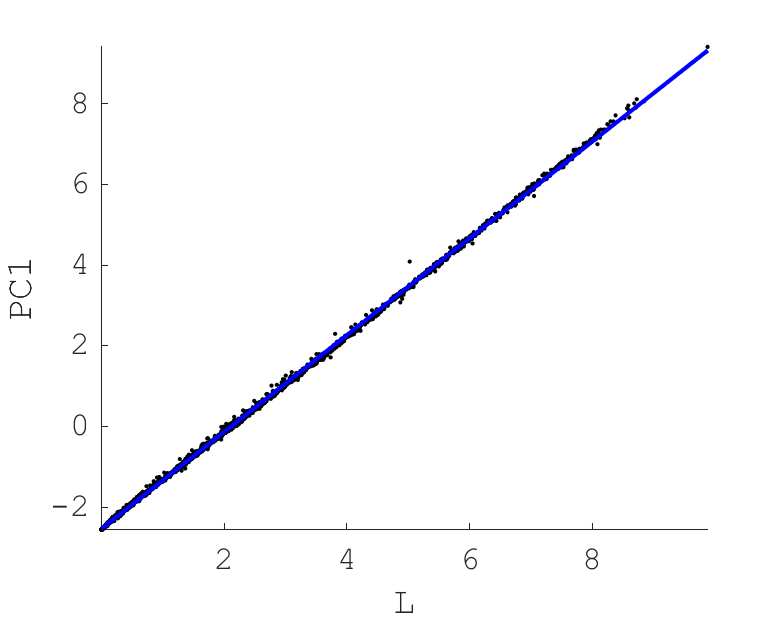
\includegraphics[max width=\textwidth]{figs/comp/melcomp_3/20.png}
 \caption{The relationship between $L$ and \gls{PC1}, showing strong correlation.}
 \label{fig:L-PC1}
\end{figure} 

\begin{figure}[htbp]
 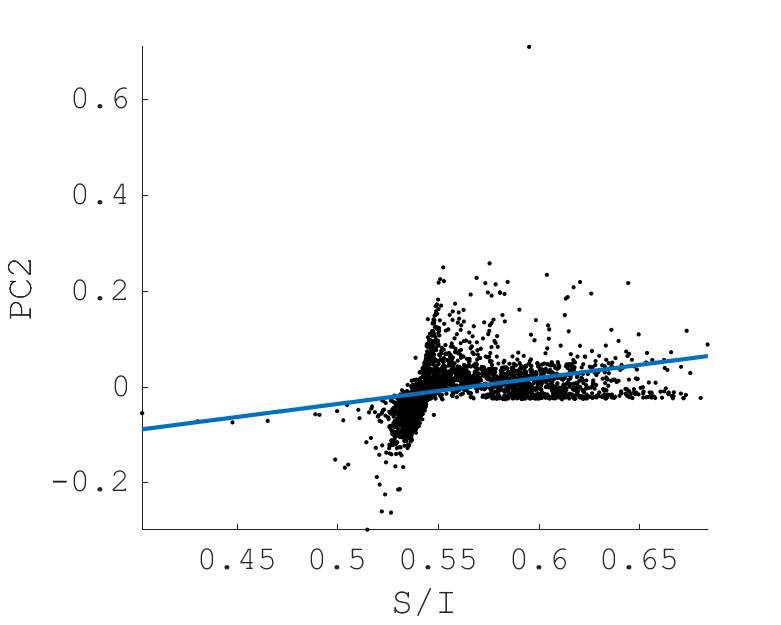
\includegraphics[max width=\textwidth]{figs/comp/melcomp_3/21.png}
 \caption{The relationship between $S/I$ and \gls{PC2}, showing weak correlation, but a clear pattern.}
 \label{fig:S/I-PC2}
\end{figure} 

\begin{figure}[htbp]
 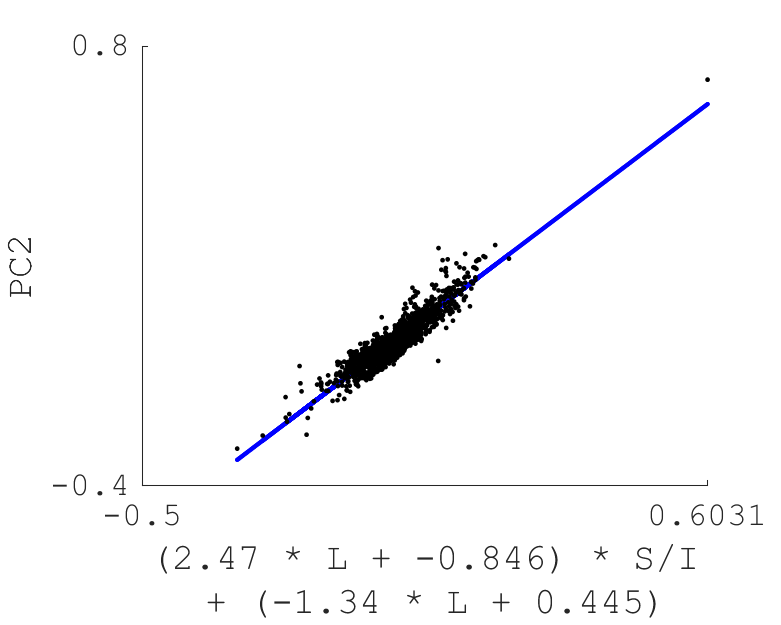
\includegraphics[max width=\textwidth]{figs/comp/melcomp_3/24.png}
 \caption{The $S/I$ signal as in Figure \ref{fig:S/I-PC2} but with a component of $L$.}
 \label{fig:withPC1}
\end{figure} 

At this point an unfortunate discrepancy between the desired function of the code and the actual function of the code was noted: whilst the desire had been to study colour signals for all surfaces under all illuminants, an averaging stage had unexpectedly averaged the signals such that computations were being performed using the average colour signal under each illuminant. 

The impact of this distinction was that the game posed by Laurence Maloney was no longer directly being queried. Instead, the question had morphed into ``Given cone catches from \emph{a single stable surface} under an unknown illuminant, guess the illuminant.'' It is still interesting to note that '$S/I$' performs very well at recovering this information however.

% Maybe I'll come back to this and maybe I won't.